\documentclass[12pt,letterpaper]{article}
\usepackage[top=2cm,left=2cm,right=2cm,bottom=2cm]{geometry}
\usepackage[utf8]{inputenc}
\usepackage[T1]{fontenc}
\usepackage{ae}               % Fonte "Almost European"
\usepackage{amsmath,amssymb}
\usepackage{setspace}
\usepackage{graphicx}
\usepackage{indentfirst}
\usepackage{url}
\usepackage{color}
\usepackage{cite}
\usepackage{gensymb}
\usepackage{subcaption}
\usepackage{hyperref}
\usepackage{epigraph}
\usepackage{mathtools}
\usepackage{mathrsfs}
\usepackage{epstopdf}

\definecolor{red}{rgb}{1.0,0.0,0.0}
\definecolor{green}{rgb}{0.01,0.75,0.24}
\definecolor{blue}{rgb}{0.0,0.0,1.0}

\newcommand{\abs}[1]{\ensuremath{\lvert #1 \rvert}}
\newcommand{\vct}[1]{{\bf #1}}
\newcommand{\eq}[1]{Eq.~(\ref{#1})}
\newcommand{\fig}[1]{Fig.~(\ref{fig:#1})}
\newcommand{\sect}[1]{Section \ref{sect:#1}}
\newcommand{\tab}[1]{Table~\ref{tab:#1}}
\newcommand{\olc}[1]{Ref.~\onlinecite{#1}}
\newcommand{\ket}[1]{| #1 \rangle}
\newcommand{\bra}[1]{\langle #1 |}
\newcommand{\expected}[1]{ \langle #1 \rangle}
\newcommand{\product}[2]{\langle #1 | #2 \rangle}
\newcommand{\pib}{\boldsymbol{\pi}}
\newcommand{\sigmab}{\boldsymbol{\sigma}}

\newcommand{\project}{\large Quantum Monte Carlo Calculations of Nucleon 
Systems and Cold atom gases \vskip 0.5cm}
\newcommand{\asu}{Physics Department \\ Arizona State University}

\begin{document}
\onehalfspacing
%\doublespace
\title{\project {\Large \textbf{Scaling and Code Performance}} \vspace{0cm}}
\author{
Project participants:\\
{\bf PIs: Kevin E. Schmidt}, Arizona State University; \\
{\bf Stefano Gandolfi}, Los Alamos National Laboratory\\
}
\date{\today}
\maketitle
\section{Scaling}
We present the scaling of our Auxiliary Field Diffusion Monte Carlo (AFDMC) 
code in several systems, but of course the 
most relevant information for this allocation is the scaling on XSEDE 
resources.

\subsection{SuperMIC}
During the current allocation (TG-PHY160027), we verified that our code scales 
strongly on SuperMIC, Fig.~\ref{fig:supermic}, up to 2560 cores (the largest 
number tested), although we intend to perform 
simulations with a maximum number of 1000 cores.

\begin{figure}[h]
   \centering
   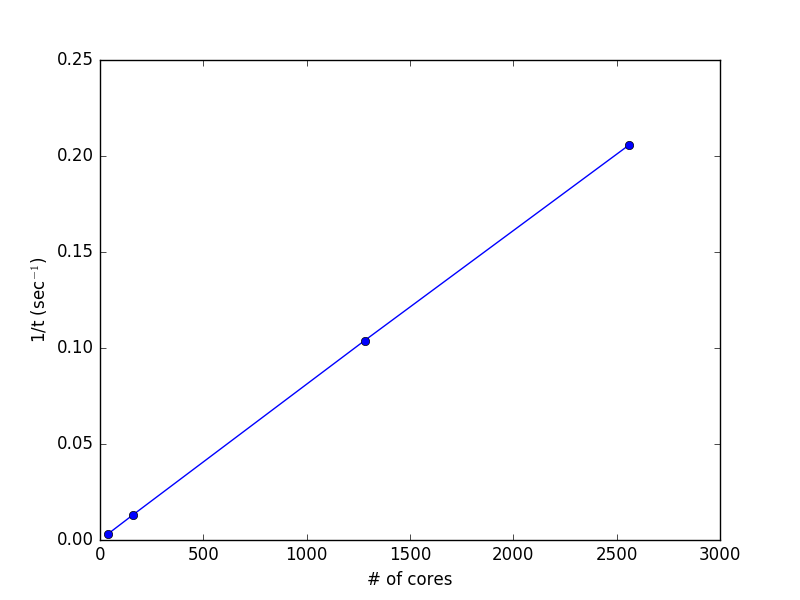
\includegraphics[width=0.5\textwidth]{supermic.png}
   \caption{Scaling on SuperMIC using the time to propagate 10,000 
   configurations of an $^{16}$O nucleus for 100 steps.}
   \label{fig:supermic}
\end{figure}

\subsection{Stampede}

We used our startup allocation (TG-PHY140003, PI Kevin Schmidt) to test the 
performance of the code on Stampede. Up to 4096 cores, the 
largest number tested, the code scales strongly.%We intend to perform 
%simulations with a maximum number of 1024 cores.

\begin{figure}[h]
   \centering
   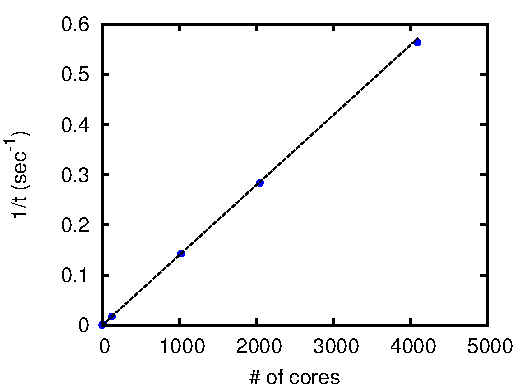
\includegraphics[width=0.5\textwidth]{stampede.pdf}
   \caption{Scaling on Stampede using the time to propagate 10,000 
   configurations of an $^{16}$O nucleus for 100 steps.}
   \label{fig:scaling}
\end{figure}

\subsection{Other systems}

Although heavy load-balancing is
involved, AFDMC shows very good strong scaling up to 96,000 cores on Edison 
at National Energy Research Scientific Computing Center (NERSC)
\footnote{Edison is a Cray XC30, with a peak performance of 2.57 
petaflops/sec, 133,824 compute cores, 357 terabytes of memory, and 7.56 
petabytes of disk.
\url{https://www.nersc.gov/users/computational-systems/edison/}
}, and
up to (at least) 24,000 cores on Mustang\footnote{
Mustang - 1,600 compute nodes, 38,400 cores, 353 TF system. 24-core AMD 
Opteron w/ InfiniBand. \url{http://www.lanl.gov/asc/tri-lab-resources.php}
}. 
We have also tested the performance on Mira at Argonne National Laboratory 
(ANL)
\footnote{
Mira, 10-petaflops IBM Blue Gene/Q system, consisting of 48 racks 786,432 
processors, and 768 terabytes of memory,
\url{https://www.alcf.anl.gov/mira}
}, with good scaling up to 128,000 cores, Fig. \ref{fig:mustang}. The code 
is very portable, and is being used extensively on Los Alamos National 
Laboratory (LANL) Institutional 
Computing resources
Wolf, Pinto and Mustang, and in the past on Lobo, Conejo and Mapache
\footnote{\url{http://www.lanl.gov/asc/tri-lab-resources.php}}.
In addition, it is being used at NERSC on Edison, Hopper and Carver, Fig. 
\ref{fig:cray}.

\begin{figure}[!htb]
\centering
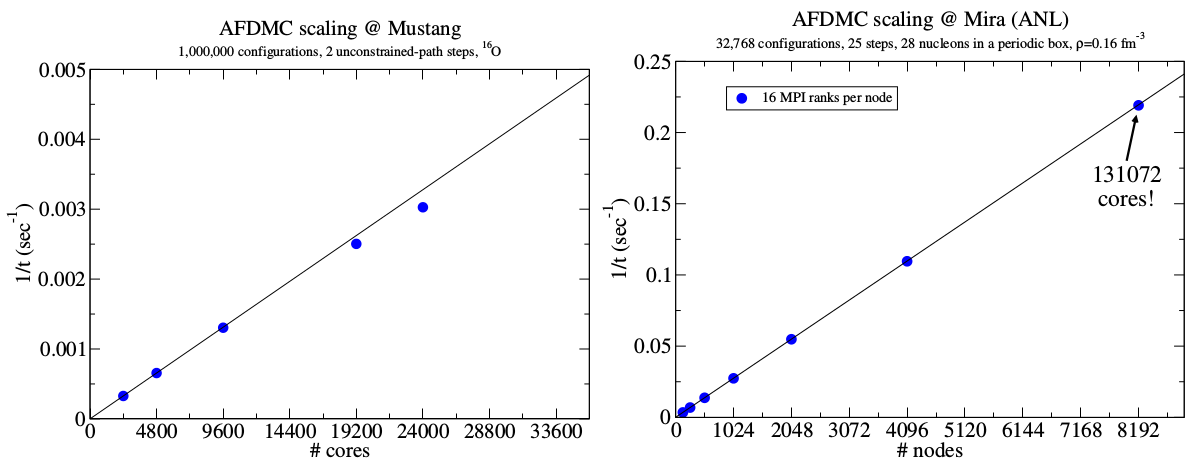
\includegraphics[width=\linewidth]{mustang.png}
\caption{Efficiency of the AFDMC code. On Mustang we tested the unconstrained-
path AFDMC
for the $^{16}$O (left panel), and the constrained-path version using fewer 
configurations on Mira for 28
nucleons in a box (right panel).}
\label{fig:mustang}
\end{figure}	

\begin{figure}[!htb]
\centering
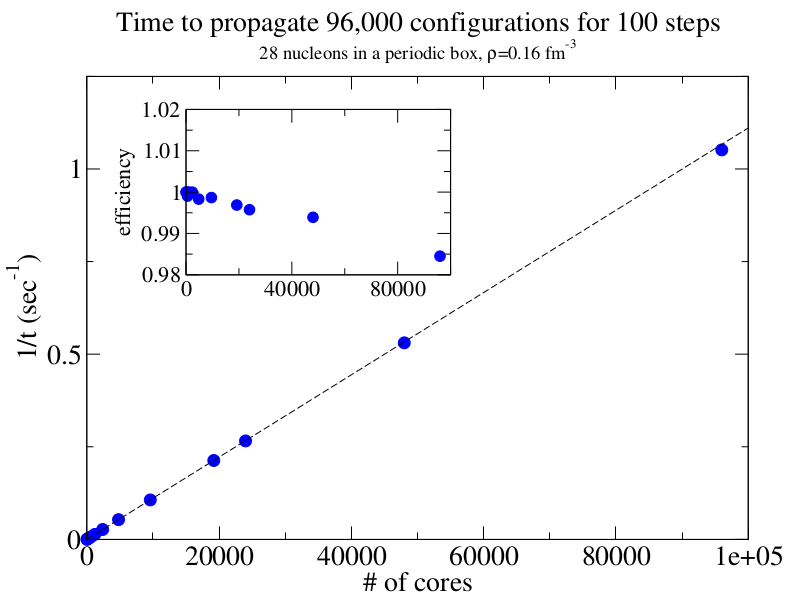
\includegraphics[width=0.5\linewidth]{cray.png}
\caption{Scaling of the AFDMC code obtained on the Cray XC30 machine at NERSC.}
\label{fig:cray}
\end{figure}	

\newpage
\section{High performance computing}

The AFDMC code is ready to run on SuperMIC, however we plan to address 
vectorization and data reuse, threading and checkpoint/restart capabilities in 
the future.

\begin{enumerate}
\item \textbf{Vectorization \& data reuse:} The MPI-only version of AFDMC 
currently shows, on average, 20\% floating point vector utilization based on 
Allinea MAP profile output, which is good, but we feel can be improved. 
During the recent Open Science Intel hackathon, using Intel vTune and 
compiler optimization reports, we were able to identify several hot spots 
and inhibitors to vectorization. Using well-placed pragmas, loop fissioning, 
and data restructuring, we were able to quickly see localized performance 
gains. We plan to continue using these tools to identify opportunities for 
increased vectorization.

\item \textbf{Threading:}
Currently, several configurations are distributed to each rank and, at each 
time step, we perform a dynamic load rebalancing since some configurations 
branch and others are removed. We plan to reduce the frequency (or need) of 
load rebalancing at each time step, by implementing an MPI+OpenMP 
programming model, so that each rank can receive a larger number of 
configurations and minimize the impact of the workload fluctuation within a 
node. The reduction in the time spent for load rebalancing and localization 
of data will significantly reduce our run time and improve our throughput.

\item \textbf{Checkpoint/restart and I/O:}
AFDMC has checkpoint/restart capabilities using POSIX calls and an 
aggregator routine written in Fortran. At user-selected intervals, state 
information is aggregated and checkpoint/restart file(s) are written, with 
aggregators determined by the number of total configurations. A full 
configuration output file can be written at user defined intervals, however it
is not written often due to the time required for I/O. The configuration 
output file can be used for additional post-processing and analysis. During 
a simulation, the observables can be calculated in two ways: they can be 
evaluated for each configuration on-the-fly, or can be saved and read in a 
separate post-processing calculation of the observables.
\end{enumerate}

\textbf{Computational Campaign:} Observables including the momentum 
distribution are calculated every several hundred steps, along with 
statistical errors. Because of the short-range nature of the diffusion at 
each step, careful attention must be used to obtain statistically 
independent samples of the proton and neutron radii. To achieve sufficient 
statistics for the energy, AFDMC requires about 100,000 steps and at least 
20,000 configurations. In the loop described above, it is necessary to 
calculate the complete wave function, $\Psi$, several times. The 
computational cost scales as $N^3$ to calculate $\Psi$, with N being the 
number of particles. The calculation of other observables (including the 
energy) adds another factor proportional to $N^2$ to the computational cost.

\newpage
\bibliographystyle{unsrt}
\bibliography{xsede}
\end{document}